\chapter{Processi e Thread}

\section{Processi}

\textbf{Processo}: è l'\textit{astrazione} di un programma in esecuzione. Il processo è l'astrazione più elementare e più importante che ci può fornire il sistema operativo. Riuscendo ad emulare il comportamento di esecuzione concorrente nonostante la presenza di una singola CPUs. \\
Un altro paio di definizioni:
\begin{itemize}[nosep]
    \item \textbf{algoritmo}: in matematica ed informatica ci si riferisce ad algoritmo ad una sequenza finita di istruzioni rigorose matematiche che hanno l'obiettivo di risolvere una determinata classe di un problema specifico o di risolvere un calcolo.
    \item \textbf{programma}: è la sequenza o l'insieme di istruzioni in liguaggio macchina che può essere eseguito.
\end{itemize}
I moderni computer possono eseguire diverse operazioni nello stesso istante. Descrivendo in maniera rigida quello che effettivamente succede, però, è che ogni CPU in \textit{ogni istante di tempo} esegue \textbf{uno e un solo} processo. Tendendo a 0 il tempo riservato a ogni singolo processo è però possibile simulare \textbf{parallelismo} definito anche come: \textbf{\textit{pseudoparallelism}}, che però va in contrasto con il vero parallelismo hardware (multi-CPUs). \\
Il \textbf{\textit{Process Model}} definisce che tutti gli eseguibili del computer, a volte includendo il sistema operativo, vengano organizzati in una serie di \textbf{processi sequenziali}. Il processo è stato definito come l'istanza di un programma in esecuizione nel quale viene anche incluso il suo \textbf{\textit{PCB}} (\textbf{\textit{Process Control Block}}). Il \textbf{PCB}, anche noto come \textit{process descriptor} è una struttura che permette di salvare tutte le informazioni che riguardano un determinato processo, ad esempio: \textit{program counter}, i registri e le variabili. Concettualmente possiamo visualizzare che ad ogni processo è associata una CPU virtuale.
\begin{boxA}
    \textcolor{red}{\textbf{\textit{Process Switching}}} \\
    È quando l'\textit{OS} cambia processo in esecuzione sulla CPU. 
\end{boxA}
Per ora considerermo che esista un'\textbf{unica CPU}. Questa assunzione non tiene normalmente conto dei moderni \textit{chip} che sono spesso multi-core. \\
Possiamo visualizzare inizialmente il processo come una tupla che contiene: il programma, degli input, degli output e uno \textbf{stato}. Un singolo processore può essere condiviso da $n$ processi con un algoritmo di \textit{scheduling} (\textit{scheduler algorithm}) che viene utilizzato per determinare quando interrompere un processo (se può farlo) e servirne un altro. \\
\begin{boxA}
    \textcolor{blue}{\textbf{Processo vs. Programma}} \\
    Un programma è qualcosa che può essere salvato su disco, statico; mentre un processo è qualcosa di dinamico e che varia ad ogni sua istanza. \\
    Un programma può essere eseguito da più processi che però sono distinti l'uno dall'altro.
\end{boxA}
La \textbf{creazione di un processo} può essere indotta da:
\begin{itemize}[nosep]
    \item inizializzazione di sistema
    \item un processo in esecuzione compie una \textit{system call} che inizializza un nuovo processo
    \item un utente richiede l'esecuzione di un nuovo processo
\end{itemize}
I processi possono essere eseguiti in \textit{foreground}, ovvero con i quali un utente può interagire, oppure in \textit{background}, che sono ``nascosti'' all'utente e rispondono a certe specifiche funzioni. Su linux sono presenti decina di processi in background, alcuni anche noti come \textit{daemons}.
\begin{boxA}
    In \textbf{UNIX} è presente una solo \textit{system call} per creare un nuovo processo: \textbf{fork}. Dopo l'esecuzione della \textit{syscall} i due processi, il padre e il figlio, hanno la stessa immagine della memoria, le stesse stringhe di environment e gli stessi file aperti. Normalmente, dopo il figlio, esegue \textbf{execve} o una \textit{system call} simile per cambiare l'area di memoria ed eseguire un nuovo programma. \\
    Alcuni implementazioni di \textbf{UNIX} condividono la sezione \textit{.text} tra i due visto che non può essere modificata. In alternativa altre implementazioni possono condividere tutta la memoria del padre, in questo caso la memoria è condivisa in maniera \textbf{\textit{copy-on-write}}, ovvero ogni volta che uno dei due vuole modificare parte della memoria, quel specifico \textit{chunck} viene copiato prima della modifica in una locazione privata della memoria
\end{boxA}
Un processo una volta creato, inizia la sua esecuzione e in un certo istante di tempo termina la sua esecuzione per una delle seguenti condizioni:
\begin{itemize}[nosep]
    \item \textit{normal exit}, il processo termina correttamente. È un tipo di condizione volontaria.
    \item \textit{error exit}, il processo termina per un errore riscontrato durante la sua esecuzione, gestito. È comunque un tipo di condizione volontaria.
    \item \textit{fatal error}, il processo termina per un errore riscontrato durante la sua esecuzione che non è stato gestito (una divisione per 0). È una condizione di interruzione involontaria.
    \item \textit{killed} da un altro processo, ovviamente involontario.
\end{itemize}
I processi, possono avere una \textbf{gerarchia}, ovvero un processo può avere solo un padre, ma $n$ figli. In alcuni sistemi un processo padre e uno figlio sono comunque sempre associati in una certa maniera.
\begin{boxA}
    In \textbf{UNIX} un processo e tutti i suoi figli sono associati in una certo modo, formando un \textit{process group}. Se un utente invia un segnale CTRL+C, questo segnale è inviato a tutti i membri della gerarchia di processi che, normalmente, sono attivi nella \textit{current window}. Individualmente, ogni processo, può catturare il segnale, ignorarlo o utilizzare l'azione di default che è quello di interrompere il processo.
\end{boxA}

\begin{wrapfigure}{R}{0.25\textwidth}
    \centering
    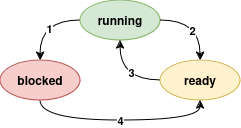
\includegraphics[width=0.25\textwidth]{img/proc_rrb}
    \caption{\textit{\textbf{Stati} di un processo}}
\end{wrapfigure}

Ogni \textbf{processo} può avere diversi \textbf{stati}:
\begin{enumerate}[nosep]
    \item \textbf{\textit{running}}: il processo sta venendo eseguito e quindi occupa la CPU in quell'istante di tempo.
    \item \textbf{\textit{ready}}: il processo è eseguibile, ma temporaneamente bloccato per permettere ad un altro processo di eseguire.
    \item \textbf{\textit{blocked}}: impossibilità di eseguire il processo finché non avviene un'azione esterna.
\end{enumerate}
Un processo può essere \textbf{bloccato} per due principali motivi: è in attesa di un input che però non è ancora disponibile oppure perché, anche se il processo è \textbf{pronto} e potrebbe essere eseguito, il sistema potrebbe aver deciso di allocare la CPU ad un altro processo. Queste due tipologie di sospensioni sono completamente diverse, nel primo caso la sospensione è \textbf{inerente} al problema, nel secondo caso è il \textit{OS}. \\
Facendo riferimento agli stati, gli stati \textbf{1} e \textbf{2} sono simili, in entrambi i casi è pronto ad eseguire, ma nel secondo stato non è c'è disponibilità di CPU, mentre il \textbf{3}rzo stato è sostanzialmente differente, il processo non può eseguire anche se la CPU è \textit{idle}. \\
Analizzando ora le transizioni da uno stato all'altro, abbiamo:
\begin{enumerate}[nosep]
    \item il processo sa che il processo non può continuare la sua esecuzione. In alcuni sistemi il processo può eseguire una \textit{syscall}, come \textbf{pause}, per entrare nello stato \textit{blocked}.
    \begin{boxA}
        In \textbf{UNIX} quando il processo deve leggere dalla \textit{pipe} o un file speciale (tipo il terminale) e non ci sono input disponibili, il processo è automaticamente bloccato.
    \end{boxA}
    \item (è gestito dallo \textit{scheduler}). Avviene quando lo \textit{scheduler} decide che il processo in esecuzione ha eseguito per troppo tempo e vuole permettere ad un altro processo di ottenere il possesso della CPU.
    \item quando tutti i processi hanno eseguito per una porzione di tempo equa, il primo processo può riprendere il possesso della CPU per eseguire nuovamente (non è sempre detto che sia il primo, dipende dallo \textit{scheduler} - esistono molti algoritmi di \textit{scheduling} che cercano di bilanciare la richiesta di utilizzo di CPU in maniera efficente (\textit{efficienty}) per il sistema e equa (\textit{fairness}) per il processo).
    \item quando l'evento esterno che il processo stava aspettando, avviene (come la scrittura su qualche input da parte di un utente). A quel punto se la CPU è in uno stato di \textit{idle} il processo eseguirà subito la transizione numero \textbf{3}, se no dovrà aspettare nello stato \textit{ready} fintanto che la CPU non tornerà disponibile.
\end{enumerate}


\begin{figure}[h]
    \centering
    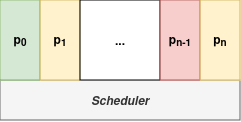
\includegraphics[width=0.25\textwidth]{img/ps}
\end{figure}

Il livello più basso del sistema operativo è lo \textit{scheduler} con tutta la varietà dei processi sopra di lui. Tutti i gestori degli \textit{interrupt} e i dettagli dei processi avviati e stoppati sono nascosti sono nascosti in quello che viene chiamato \textit{scheduler}, mentre il resto del sistema operativo è strutturato e rappresentato tramite l'astrazione di un processo. \textbf{Molti pochi dei reali sistemi operativi sono strutturati in questa maniera}. \\

Per implementare il \textbf{\textit{process model}}, il sistema operativo deve mantenere in memoria una tabella (un \textit{array} di strutture), chiamata \textbf{\textit{process table}}, dove ogni processo è una voce di questa tabella (è chiamata anche \textbf{PCB}). Al suo interno sono salvati informazioni (Tabella \ref{tab:pcb}) che permettono, al processo, di passare dallo stato di \textit{ready} a quello di \textit{running} (e viceversa) come se non si fosse mai interrorto.

\begin{center}
    \begin{tabular}{ | c | c | c | } \hline
        \textbf{gestione di processi} & \textbf{gestione della memoria} & \textbf{gestione dei file} \\ \hline
        registri & puntatore al \textit{text segment} & \textit{root directory} \\ \hline
        \textit{program counter} & puntatore al \textit{data segment} & \textit{working directory} \\ \hline
        \textit{program status word} & puntatore al \textit{stack segment} & \textit{file descriptor} \\ \hline
        \textit{stack pointer} & & \textit{user id} \\ \hline
        \textit{process state} & & \textit{group id} \\ \hline
        priorità & & \\ \hline
        \textit{scheduling param} & & \\ \hline
        \textit{process id} & & \\ \hline
        processo padre & & \\ \hline
        \textit{process group} & & \\ \hline
        \textit{signal} (CTRL+C) & & \\ \hline
        \textit{timestamp} di inizio & & \\ \hline
        \textit{CPU time} & & \\ \hline
        \textit{CPU time} dei figli & & \\ \hline
    \end{tabular}
    \label{tab:pcb}
    \captionof{table}{Contenuto del \textit{Process Control Block}}
\end{center}

Se consideriamo di avere un processo $p_0$ che però per l'$80\%$ della sua esecuzione è in attesa di un I/O, allora quella CPU verrà utilizzata solo al $20\%$. Come possiamo ottimizzare il tempo di \textit{idle} della CPU. Se dovessimo mettere altri 4 processi $p_1, p_2, p_3, p_4$ che hanno lo stesso pattern di esecuzione di $p_0$, idealmente avremo che la CPU verrebbe utilizzata al $100\%$, ma un modello del genere sarebbe non realisticamente ottimistico, perché si aspetta che i 5 processi non aspettino l'I/O nello stesso istante in maniera sequenziale. Un modello per avere \textbf{pseudo-parallelismo} è quello di osservare l'utilizzazione della CPU da un punto di vista probabilistico. Supponiamo che il processo $p$ spende una frazione di $p$ in attesa del completamento di un'azione di I/O, la probabilità che $n$ processi aspettino l'azione di I/O is $p^n$. Allora l'utilizzazione della CPU è data dalla formula:
\begin{center}
    $CPU_{utlization} = 1 - p^n$
\end{center}

\begin{figure}[h]
    \centering
    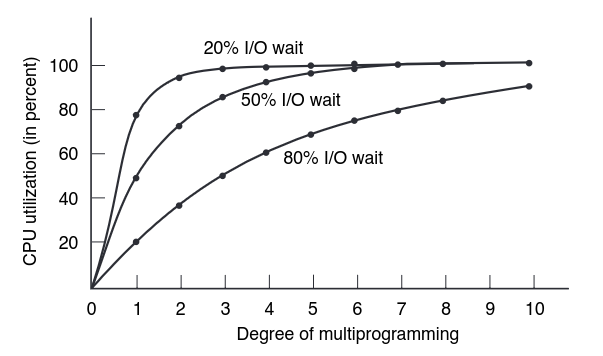
\includegraphics[width=0.45\textwidth]{img/deg_multiprog}
    \caption{\textit{Funzione di utilizzazione della CPU}}
    \label{fig:deg_multip}
\end{figure}

La Figura \ref{fig:deg_multip} ci mostra come a diversi valori della frazione di $p$ per l'attesa dell'I/O, l'utilizzazione della CPU sia funzione del numero di processi in memoria $n$, questa condizione è nota come \textbf{\textit{degree of multiprogramming}}. \\
Dalla figura è chiaro che se i processi spendono l'$80\%$ del loro tempo di esecuzione in attesa, ci devono essere in memoria almeno $n=10$ per avere un \textit{CPU waste} del $10\%$. \\
È giusto specificare che quello che descrive il modello probabilistico è un'approssimazione. Assume, implicitamente, che i gli $n$ processi sono indipendenti, il che significa che è accettabile per un sistema con 5 processi in memoria di averne 3 di questi in esecuzione (\textit{running}) e due in attesa (\textit{ready}), ma con un'unica CPU è impossibile avere 3 processi attivi contemporaneamente. Un modello più accurato è possibile costruirlo utilizzando la teoria delle code (\textbf{\textit{queueing theory}}).